\documentclass[tikz,border=2pt]{standalone}
\usepackage{amsmath}
\usetikzlibrary{arrows.meta}
\begin{document}
% Sample path of L(t) on [0,10] (arrivals 1,2,4,8; departures 3,6,7). Arrivals see L(A_k-) = 0,1,1,0,
% so the arrival fractions are 1/2, 1/2, 0 (green), against the time fractions 0.2, 0.5, 0.3 (grey).
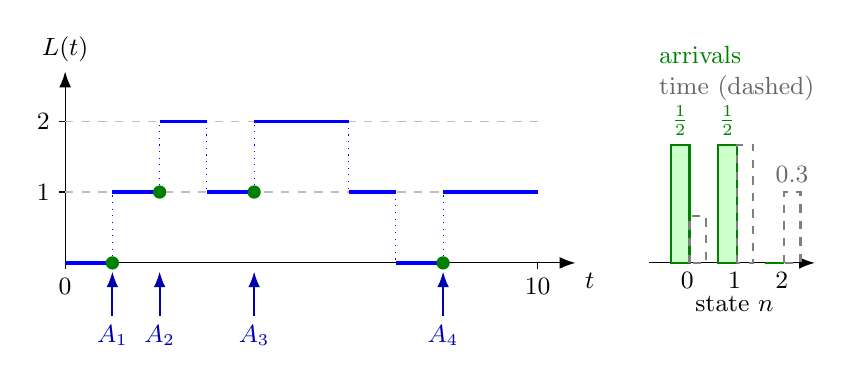
\begin{tikzpicture}[font=\small, >={Latex[length=2mm]}, x=0.6cm, y=0.9cm]
  % ---------- sample path ----------
  \draw[->] (0,0) -- (10.8,0) node[anchor=north west] {$t$};
  \draw[->] (0,0) -- (0,2.7) node[anchor=south] {$L(t)$};
  \foreach \x in {0,10} \draw (\x,0) -- (\x,-0.08) node[anchor=north] {$\x$};
  \foreach \y in {1,2} {
    \draw (0,\y) -- (-0.12,\y) node[anchor=east] {$\y$};
    \draw[gray!50, thin, dashed] (0,\y) -- (10,\y);
  }
  \draw[blue, very thick] (0,0) -- (1,0) (1,1) -- (2,1) (2,2) -- (3,2) (3,1) -- (4,1)
    (4,2) -- (6,2) (6,1) -- (7,1) (7,0) -- (8,0) (8,1) -- (10,1);
  \draw[blue, thin, dotted] (1,0) -- (1,1) (2,1) -- (2,2) (3,2) -- (3,1) (4,1) -- (4,2)
    (6,2) -- (6,1) (7,1) -- (7,0) (8,0) -- (8,1);
  % arrivals and what they see
  \foreach \a/\s/\k in {1/0/1,2/1/2,4/1/3,8/0/4} {
    \draw[->, blue!70!black, thick] (\a,-0.75) -- (\a,-0.12);
    \node[blue!70!black, anchor=north] at (\a,-0.75) {$A_{\k}$};
    \fill[green!50!black] (\a,\s) circle (2.4pt);
  }
  % ---------- arrival fractions against time fractions ----------
  \begin{scope}[xshift=7.6cm, y=3cm]
    \draw[->] (-0.3,0) -- (3.2,0);
    \foreach \n/\v/\p/\lab in {0/0.5/0.2/{1/2},1/0.5/0.5/{1/2},2/0/0.3/0} {
      \fill[green!20] (\n+0.15,0) rectangle (\n+0.55,\v);
      \draw[green!50!black, thick] (\n+0.15,0) rectangle (\n+0.55,\v);
      \draw[gray, thick, dashed] (\n+0.55,0) rectangle (\n+0.9,\p);
      \node[anchor=north] at (\n+0.5,0) {$\n$};
    }
    \node[green!50!black, anchor=south] at (0.35,0.5) {$\tfrac{1}{2}$};
    \node[green!50!black, anchor=south] at (1.35,0.5) {$\tfrac{1}{2}$};
    \node[gray!80!black, anchor=south] at (2.72,0.3) {$0.3$};
    \node[anchor=north] at (1.5,-0.1) {state $n$};
    \node[green!50!black, anchor=west] at (-0.3,0.88) {arrivals};
    \node[gray!80!black, anchor=west] at (-0.3,0.74) {time (dashed)};
  \end{scope}
\end{tikzpicture}
\end{document}
